\section{Kết quả}\label{sec:results}
% Mọi con số lấy từ data/results/analysis/main (gói code/analysis/ tại thẻ prereg-v1-analysis) qua report-data
% build. Kết cục ghi đúng như gói phân tích đọc theo bản đăng ký.

\subsection{Hồi cứu (RQ1, RQ2)}\label{sec:retrospective}

Bảng~\ref{tab:lifecycle} phân bổ \NumCommits{} commit và \NumLinesChanged{} dòng thay đổi
theo khâu. Công việc dồn vào hai đợt: giữa tháng 9, khi backend, frontend, kho dữ liệu và phần đánh giá được
dựng, và đầu tháng 10, khi các tính năng tài khoản và tổ chức được thêm (Hình~\ref{fig:lifecycle}). Khâu kiểm
thử chiếm tỉ lệ commit lớn nhất (\NumStageTestCommitsPct{}\%) nhưng chỉ \NumStageTestLinesPct{}\% số dòng.
Nguyên nhân là cách gán khâu: các plan của ViPharmind yêu cầu viết test trước, nên nhiều commit \texttt{feat}
thêm nhiều dòng test hơn dòng mã, và \NumFeatInTestStage{} trong \NumCommitsFeat{} commit \texttt{feat} được
gán vào khâu kiểm thử. Theo số dòng, dữ liệu (\NumStageDataLinesPct{}\%) và backend
(\NumStageBackendLinesPct{}\%) lớn nhất. Git không cho biết dòng nào do AI viết; nhận định ``AI tham gia mọi
khâu'' dựa trên lời khai của tác giả dự án và phần nhật ký phiên còn lại (Phụ lục~\ref{sec:sessions}).

\begin{table}[H]
\centering\small
\caption{Commit và dòng thay đổi theo khâu của vòng đời}\label{tab:lifecycle}
\begin{tabular}{lrrrr}
\toprule
Khâu & Commit & \% commit & Dòng thay đổi & \% dòng \\
\midrule
nghiên cứu và đánh giá & 88 & 17,4 & 46.772 & 8,2 \\
dữ liệu & 68 & 13,5 & 166.015 & 29,0 \\
mã backend & 86 & 17,0 & 162.944 & 28,4 \\
mã frontend & 49 & 9,7 & 91.362 & 15,9 \\
kiểm thử & 161 & 31,9 & 79.777 & 13,9 \\
triển khai & 8 & 1,6 & 1.877 & 0,3 \\
tài liệu & 34 & 6,7 & 23.062 & 4,0 \\
khác & 11 & 2,2 & 1.552 & 0,3 \\
\midrule
Tổng & 505 &  & 573.361 &  \\
\bottomrule
\end{tabular}

\end{table}

\begin{figure}[H]
\centering
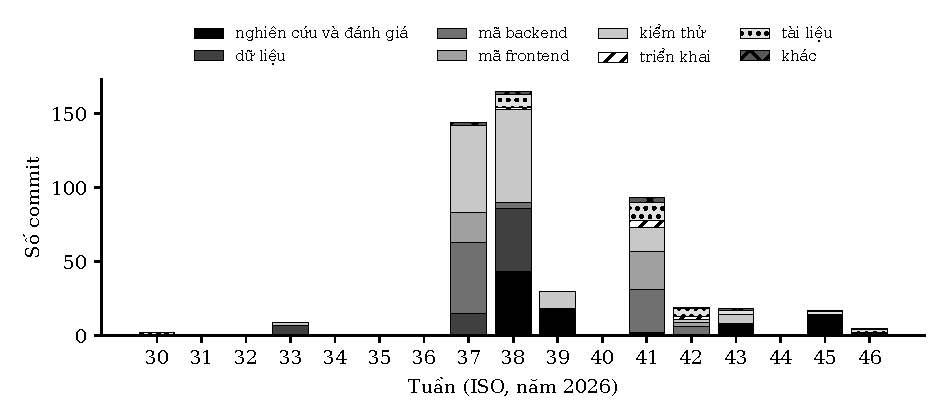
\includegraphics[width=0.8\linewidth]{generated/figures/lifecycle_by_week.pdf}
\caption{Số commit theo tuần và theo khâu}\label{fig:lifecycle}
\end{figure}

Theo quy tắc nối ở mục~\ref{sec:method}, \NumFeatWithPlan{} trong
\NumCommitsFeat{} commit \texttt{feat} (\NumFeatWithPlanPct{}\%) có plan đi trước. Quy tắc đúng ở
\NumLinkCorrect{} trên \NumLinkChecked{} commit kiểm tay (\NumLinkCorrectPct{}\%); trong các lần sai,
\NumLinkFalsePositive{} lần nối thừa và \NumLinkFalseNegative{} lần bỏ sót. Vì sai lệch nghiêng về nối thừa,
tỉ lệ \NumFeatWithPlanPct{}\% nhiều khả năng là cận trên. Dù vậy, phần lớn commit tính năng của ViPharmind đi
sau một plan có nêu file mà chúng chạm: quy trình mà nhánh theo đặc tả của thực nghiệm tái hiện.

Commit \texttt{feat} có plan đi trước có trung bình \NumReworkWithPlanMean{} commit sửa
lại trong 14 ngày, \NumReworkWithPlanSharePct{}\% có ít nhất một lần sửa; nhóm không có plan có trung bình
\NumReworkWithoutPlanMean{}, tỉ lệ \NumReworkWithoutPlanSharePct{}\% (Bảng~\ref{tab:rework}). Hai nhóm gần như
nhau. Nhóm không có plan chỉ có \NumFeatWithoutPlan{} commit và khác nhóm kia về thời điểm và loại việc, nên đây
là quan sát, không phải quan hệ nhân quả; câu hỏi nhân quả được trả lời bằng thực nghiệm dưới đây.

\begin{table}[H]
\centering\small
\caption{Số commit sửa lại trong 14 ngày sau mỗi commit \texttt{feat}}\label{tab:rework}
\begin{tabular}{lrrrr}
\toprule
Nhóm & Số \texttt{feat} & Trung bình & Trung vị & \% có sửa lại \\
\midrule
Có plan đi trước & 196 & 2,26 & 2 & 79,6 \\
Không có plan & 25 & 2,00 & 2 & 76,0 \\
\bottomrule
\end{tabular}

\end{table}

\subsection{Thực nghiệm chính (RQ3--RQ6)}\label{sec:data-collected}

Ba nhóm \texttt{claude-sonnet}, \texttt{claude-opus} và \texttt{codex-luna} chạy đủ \NumResRunsPerCohort{}
lượt mỗi nhóm, tổng \NumResRuns{} lượt hợp lệ. Không lượt nào hết giờ, thoát lỗi hay bị loại vì lỗi bộ chạy.
Mỗi (nhiệm vụ, cách làm) có đúng một mã băm đề bài ở cả \NumResPromptCells{} ô, và mỗi nhóm chỉ gặp một phiên
bản công cụ. Mọi lượt theo đặc tả để lại cả \texttt{docs/design.md} lẫn \texttt{docs/plan.md}; không lượt vibe
nào viết hai file này, nên can thiệp được thực hiện đúng.

Nhóm \texttt{agy-gemini} bị loại: cả bốn tài khoản Antigravity hết hạn mức tuần khi nhóm này mới xong
\NumResAgyDone{} trên \NumResRunsPerCohort{} lượt. Số đếm thô của phần đã xong được xem trước quyết định loại
(Phụ lục~\ref{app:deviations}), nên quyết định này không hoàn toàn độc lập với kết quả. RQ4 vì vậy chỉ còn hai
công cụ.

Bảng~\ref{tab:main} và Hình~\ref{fig:by-cohort} tóm tắt tỉ lệ đạt theo nhóm và tầng.

\begin{table}[H]
\centering\small
\caption{Tỉ lệ đạt theo nhóm, tầng và cách làm. Hiệu số là đặc tả trừ vibe (đpt), KTC 95\% bootstrap theo
nhiệm vụ. Tầng vừa và tầng lớn dưới sáu nhiệm vụ nên KTC chỉ để tham khảo.}
\label{tab:main}
\begin{tabular}{llrrlr}
\toprule
Nhóm & Tầng & Đặc tả (\%) & Vibe (\%) & Hiệu số (đpt) [KTC 95\%] & Kết cục \\
\midrule
\texttt{claude-sonnet} & nhỏ & 89 & 91 & -2,2 [-6,7; 0,0] & chưa rõ \\
\texttt{claude-sonnet} & vừa & 100 & 93 & 6,7 [0,0; 20,0] & chưa rõ \\
\texttt{claude-sonnet} & lớn & 67 & 78 & -11,1 [-33,3; 0,0] & chưa rõ \\
\texttt{claude-opus} & nhỏ & 84 & 89 & -4,4 [-17,8; 6,7] & chưa rõ \\
\texttt{claude-opus} & vừa & 100 & 100 & 0,0 [0,0; 0,0] & chưa rõ \\
\texttt{claude-opus} & lớn & 78 & 89 & -11,1 [-33,3; 0,0] & chưa rõ \\
\texttt{codex-luna} & nhỏ & 78 & 71 & 6,7 [-4,4; 17,8] & chưa rõ \\
\texttt{codex-luna} & vừa & 60 & 73 & -13,3 [-40,0; 0,0] & chưa rõ \\
\texttt{codex-luna} & lớn & 44 & 11 & 33,3 [33,3; 33,3] & ủng hộ \\
gộp ba nhóm & nhỏ &  &  & 0,0 [-4,4; 4,4] &  \\
gộp ba nhóm & vừa &  &  & -2,2 [-13,3; 6,7] &  \\
gộp ba nhóm & lớn &  &  & 3,7 [0,0; 11,1] &  \\
\bottomrule
\end{tabular}

\end{table}

\begin{figure}[H]
\centering
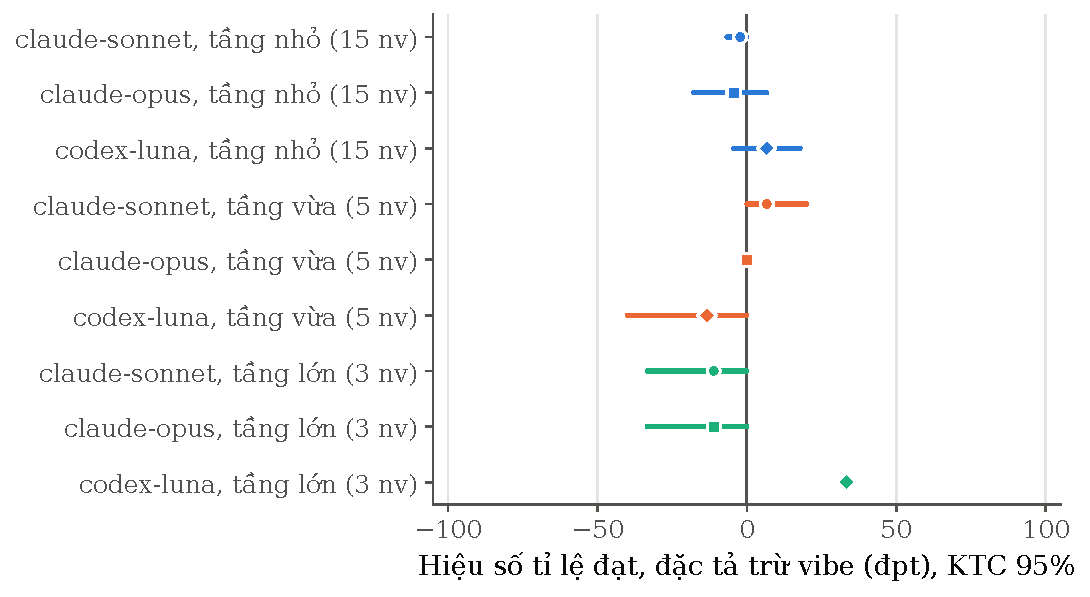
\includegraphics[width=0.8\linewidth]{generated/figures/pass_diff_by_cohort.pdf}
\caption{Hiệu số tỉ lệ đạt (đặc tả trừ vibe) theo nhóm và tầng, kèm KTC 95\%}
\label{fig:by-cohort}
\end{figure}

Với phép thử xác nhận H1 (\texttt{claude-sonnet}, tầng nhỏ), nhánh theo đặc tả đạt
\NumResHOneSpecPct{}\%, nhánh vibe đạt \NumResHOneVibePct{}\%, hiệu số \NumResHOneEstPp{} đpt, KTC
[\NumResHOneLowPp{}; \NumResHOneHighPp{}]. KTC chứa 0 nên H1 \textbf{chưa kết luận được}. KTC không chứa giá trị
dương nào, nên dữ liệu không ủng hộ một lợi ích đáng kể; tuy vậy, với \NumTasks{} nhiệm vụ, chưa loại được một
lợi ích nhỏ. Ba lần lặp của cùng một (nhiệm vụ, cách làm) cho kết quả khác nhau ở \NumResVarDisagree{} trên
\NumResVarCells{} ô (\NumResVarDisagreePct{}\%) của phép thử này, cho thấy biến thiên giữa các lần chạy là đáng
kể.

Đổi công cụ cũng không cho hướng rõ ràng (RQ4). Ở tầng nhỏ, hiệu số của \texttt{claude-opus} là \NumResOpusSmallDiffPp{} đpt và của
\texttt{codex-luna} là \NumResCodexSmallDiffPp{} đpt; cả hai KTC đều chứa 0. Hướng hiệu số âm với hai mô hình
Claude và dương với Codex. Ô duy nhất có kết cục ``ủng hộ'' là \texttt{codex-luna} tầng lớn: đặc tả
\NumResCodexLargeSpecPct{}\%, vibe \NumResCodexLargeVibePct{}\%. KTC của ô này suy biến thành một điểm vì cả ba
nhiệm vụ cho cùng hiệu số, và gói phân tích đếm \NumResSecondaryComparisons{} phép so phụ không hiệu chỉnh, nên
ô này cần được đọc thận trọng.

Đổi sang mô hình mạnh hơn cũng không làm thay đổi bức tranh (RQ5, H4). Ở tầng nhỏ, hiệu của hai hiệu số (Sonnet trừ Opus) là
\NumResHFourDiffOfDiffsPp{} đpt, KTC [\NumResHFourDiffOfDiffsLowPp{}; \NumResHFourDiffOfDiffsHighPp{}]; H4
\textbf{chưa kết luận được} ở cả ba tầng. Sonnet theo đặc tả và Opus vibe có cùng ước lượng điểm (hiệu
\NumResHFourSonnetSpecOpusVibePp{} đpt, KTC [\NumResHFourSonnetSpecOpusVibeLowPp{};
\NumResHFourSonnetSpecOpusVibeHighPp{}]) với chi phí bằng \NumResHFourCostRatioPct{}\%. Điều này phản ánh việc cả
hai mô hình đã gần trần ở tầng nhỏ, không cho thấy quy trình nâng mô hình yếu lên.

Hiệu số cũng không tăng rõ theo kích thước nhiệm vụ (RQ6, H5). Hiệu số gộp ba nhóm là \NumResHFiveLargePp{} đpt ở tầng lớn và
\NumResHFiveSmallPp{} đpt ở tầng nhỏ; hiệu của hai giá trị này là \NumResHFiveEstPp{} đpt, KTC
[\NumResHFiveLowPp{}; \NumResHFiveHighPp{}]. Hệ số tương tác (cách làm $\times$ log số dòng) của mô hình hỗn hợp
là \NumResHFiveCoef{} trên thang logit, KTC [\NumResHFiveCoefLow{}; \NumResHFiveCoefHigh{}]. H5
\textbf{chưa kết luận được}. Hình~\ref{fig:effect-size} cho thấy hiệu số của phần lớn nhiệm vụ bằng không; các
nhiệm vụ lệch nằm ở cả hai phía và ở mọi cỡ; riêng ba nhiệm vụ tầng lớn của Codex đều lệch về phía đặc tả.

\begin{figure}[H]
\centering
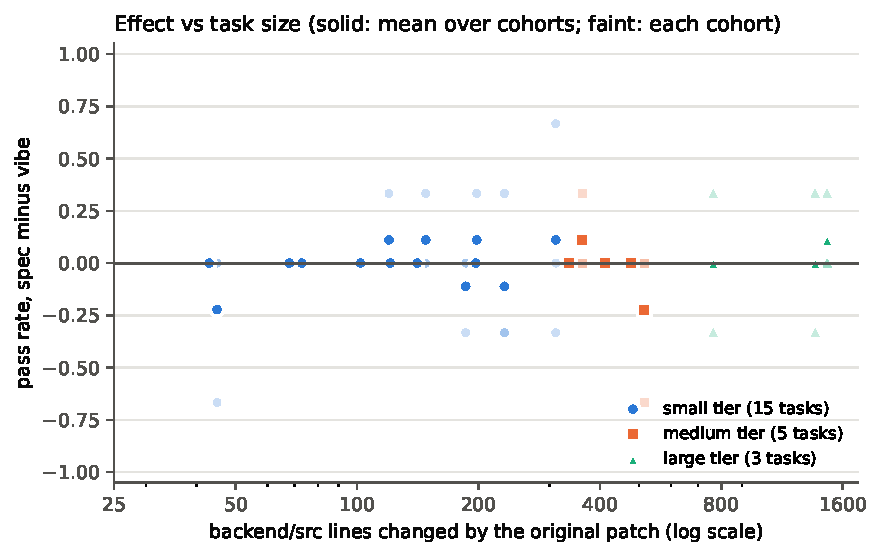
\includegraphics[width=0.78\linewidth]{generated/figures/effect_vs_size.pdf}
\caption{Hiệu số tỉ lệ đạt theo số dòng của bản vá gốc; mỗi điểm là một nhiệm vụ của một nhóm}
\label{fig:effect-size}
\end{figure}

Các phân tích độ nhạy không làm đổi kết luận. Bỏ \NumResSensUrlRuns{} lượt của nhiệm vụ có đường dẫn tới mã gốc trong nhật ký, H1 thành
\NumResSensUrlEstPp{} đpt [\NumResSensUrlLowPp{}; \NumResSensUrlHighPp{}]. Bỏ cặp nhiệm vụ chung commit
(\texttt{f08}, \texttt{t03}), H5 thành \NumResSensOverlapEstPp{} đpt [\NumResSensOverlapLowPp{};
\NumResSensOverlapHighPp{}]. Bỏ \NumResSensPytestRuns{} lượt sửa cấu hình \texttt{pytest}, hoặc dùng số dòng
được chấm thay số dòng của bản vá gốc (hệ số \NumResHFiveGradedCoef{} [\NumResHFiveGradedLow{};
\NumResHFiveGradedHigh{}]), kết cục cũng không đổi.

Về chi phí, H2 \textbf{được ủng hộ} ở mọi nhóm và tầng (Bảng~\ref{tab:secondary}). Nhánh theo đặc tả dùng gấp
\NumResTokenRatioMin{} đến \NumResTokenRatioMax{} lần token và gấp \NumResWallRatioMin{} đến
\NumResWallRatioMax{} lần thời gian của nhánh vibe; mức thêm thấp nhất ở Opus (\NumResOpusTokenRatio{} lần
token), cao nhất ở Codex (\NumResCodexTokenRatio{} lần). Vì tỉ lệ đạt gần như nhau, chi phí quy đổi cho một
lượt đạt cao hơn ở nhánh theo đặc tả trong mọi ô của hai mô hình Claude (Bảng~\ref{tab:cost}); riêng Codex tầng
lớn thì ngược lại, vì nhánh vibe gần như không đạt.

H3 cho kết quả lẫn lộn. Về lỗi tĩnh, nhánh theo đặc tả có nhiều lỗi hơn ở hai ô (\texttt{claude-sonnet} tầng
vừa, \texttt{codex-luna} tầng nhỏ). Ở \texttt{codex-luna} tầng lớn thì ngược lại: trung bình
\NumResCodexLargeStaticSpec{} so với \NumResCodexLargeStaticVibe{} lỗi tĩnh mỗi lượt, và
\NumResCodexLargeRegSpecPct{}\% so với \NumResCodexLargeRegVibePct{}\% lượt làm hỏng test cũ. Hai mô hình Claude
gần như không làm hỏng test cũ ở cách làm nào. Về chỉ số bảo trì, nhánh theo đặc tả không kém hơn quá 5 điểm ở
hầu hết các ô.

\begin{table}[H]
\centering\scriptsize\setlength{\tabcolsep}{3pt}
\caption{Chi phí và chất lượng, mỗi ô là trung bình nhánh theo đặc tả / nhánh vibe. Token gồm cả token đọc
cache. Lỗi tĩnh là số lỗi ruff và pyrefly trên các file bị đổi. Hồi quy là tỉ lệ lượt làm hỏng ít nhất một
test cũ. $\Delta$MI là thay đổi chỉ số bảo trì so với commit cha.}
\label{tab:secondary}
\begin{tabular}{llrrlrlrlrl}
\toprule
Nhóm & Tầng & Token (triệu) & Phút & H2 & Lỗi static analysis & H3a & Regression (\%) & H3b & $\Delta$MI & H3c \\
\midrule
\texttt{claude-sonnet} & nhỏ & 0,41 / 0,21 & 3,3 / 1,0 & ủng hộ & 1,3 / 0,6 & chưa rõ & 0 / 0 & chưa rõ & -1,1 / -1,6 & ủng hộ \\
\texttt{claude-sonnet} & vừa & 1,22 / 0,35 & 7,9 / 2,2 & ủng hộ & 2,0 / 0,2 & trái & 0 / 0 & chưa rõ & -5,0 / -5,6 & chưa rõ \\
\texttt{claude-sonnet} & lớn & 10,19 / 5,37 & 28,2 / 13,6 & ủng hộ & 2,4 / 1,3 & chưa rõ & 0 / 0 & chưa rõ & -0,5 / -2,8 & ủng hộ \\
\texttt{claude-opus} & nhỏ & 0,93 / 0,48 & 5,7 / 3,0 & ủng hộ & 0,3 / 0,0 & chưa rõ & 7 / 7 & chưa rõ & 3,0 / 2,6 & ủng hộ \\
\texttt{claude-opus} & vừa & 1,97 / 1,13 & 11,7 / 7,2 & ủng hộ & 0,0 / 0,2 & chưa rõ & 0 / 0 & chưa rõ & -2,5 / -2,8 & ủng hộ \\
\texttt{claude-opus} & lớn & 12,76 / 11,14 & 32,1 / 22,5 & ủng hộ & 0,0 / 0,0 & chưa rõ & 0 / 0 & chưa rõ & -0,6 / -1,0 & ủng hộ \\
\texttt{codex-luna} & nhỏ & 0,73 / 0,31 & 5,0 / 1,6 & ủng hộ & 3,2 / 1,0 & trái & 7 / 4 & chưa rõ & -2,9 / -2,4 & ủng hộ \\
\texttt{codex-luna} & vừa & 1,55 / 0,54 & 8,8 / 2,6 & ủng hộ & 8,7 / 12,9 & chưa rõ & 0 / 0 & chưa rõ & -6,5 / -9,6 & ủng hộ \\
\texttt{codex-luna} & lớn & 6,69 / 3,32 & 21,7 / 8,5 & ủng hộ & 35,1 / 74,9 & ủng hộ & 0 / 78 & ủng hộ & -3,2 / -4,3 & ủng hộ \\
\bottomrule
\end{tabular}

\end{table}

\begin{table}[H]
\centering\small
\caption{Chi phí quy đổi theo giá API cho một lượt đạt (USD); với \texttt{codex-luna} là khoảng từ cận dưới
tới cận trên của giá}
\label{tab:cost}
\begin{tabular}{llrr}
\toprule
Nhóm & Tầng & Đặc tả (USD) & Vibe (USD) \\
\midrule
\texttt{claude-sonnet} & nhỏ & 0,26 & 0,13 \\
\texttt{claude-sonnet} & vừa & 0,55 & 0,26 \\
\texttt{claude-sonnet} & lớn & 3,96 & 1,92 \\
\texttt{claude-opus} & nhỏ & 0,99 & 0,59 \\
\texttt{claude-opus} & vừa & 1,64 & 1,02 \\
\texttt{claude-opus} & lớn & 7,71 & 5,71 \\
\texttt{codex-luna} & nhỏ & 0,02--0,03 & 0,01--0,02 \\
\texttt{codex-luna} & vừa & 0,05--0,09 & 0,02--0,03 \\
\texttt{codex-luna} & lớn & 0,21--0,40 & 0,46--0,87 \\
\bottomrule
\end{tabular}

\end{table}

Khác biệt rõ nhất giữa hai cách làm là test do tác tử tự viết (Bảng~\ref{tab:tests}). Nhánh theo đặc tả viết
test ở \NumResSonnetSpecTestsAnyPct{}--\NumResCodexSpecTestsAnyPct{}\% số lượt, chạy qua
\NumResSonnetSpecCovPct{}--\NumResOpusSpecCovPct{}\% số dòng mới. Nhánh vibe khác nhau theo công cụ: Codex không
viết test nào (\NumResCodexVibeTestsAnyPct{}\%) và hầu như không chạy \texttt{pytest}
(\NumResCodexVibePytestPct{}\% số lượt), Sonnet viết test ở \NumResSonnetVibeTestsAnyPct{}\% số lượt, còn Opus
tự viết test ở \NumResOpusVibeTestsAnyPct{}\% số lượt dù không được yêu cầu. Phần chênh này là hệ quả trực tiếp
của lời dặn và cho thấy tác tử làm đúng quy trình. Test ẩn không thưởng cho phần test này: tỉ lệ đạt của hai
nhánh gần như nhau.

\begin{table}[H]
\centering\footnotesize\setlength{\tabcolsep}{4pt}
\caption{Test do tác tử viết, theo nhóm và cách làm (mọi tầng). Độ phủ là tỉ lệ dòng mới ở
\texttt{backend/src} được test của chính tác tử chạy qua, tính 0 khi lượt không viết test.}
\label{tab:tests}
\begin{tabular}{llrrrrr}
\toprule
Nhóm & Cách làm & Lượt & Chạy \texttt{pytest} (\%) & Viết test (\%) & Test mới/lượt & Phủ dòng mới (\%) \\
\midrule
\texttt{claude-sonnet} & đặc tả & 69 & 100 & 72 & 7,3 & 50 \\
\texttt{claude-sonnet} & vibe & 69 & 64 & 7 & 0,3 & 4 \\
\texttt{claude-opus} & đặc tả & 69 & 100 & 77 & 11,2 & 55 \\
\texttt{claude-opus} & vibe & 69 & 100 & 52 & 3,5 & 37 \\
\texttt{codex-luna} & đặc tả & 69 & 100 & 78 & 3,7 & 50 \\
\texttt{codex-luna} & vibe & 69 & 6 & 0 & 0,0 & 0 \\
\bottomrule
\end{tabular}

\end{table}

\subsection{Nguyên nhân thất bại và đề sơ sài}

Hai người gán nhãn độc lập \NumLabRuns{} lượt không đạt của hai nhóm Claude (\NumLabSpecRuns{} theo đặc tả,
\NumLabVibeRuns{} vibe), đồng ý ở \NumLabAgree{}/\NumLabRuns{} lượt, kappa \NumLabKappa{}; \NumLabAdjudicated{}
lượt lệch được phân xử (Bảng~\ref{tab:labels}). \NumLabOutside{} lượt hỏng không do logic tác tử tự viết:
\NumLabDeBaiThieuTotal{} vì test ẩn kiểm chi tiết đề không chốt, \NumLabSaiApiCoSanTotal{} vì nối sai với mã có
sẵn. Hai loại này chiếm tỉ lệ gần như nhau ở hai nhánh (\NumLabOutsideSpecPct{}\% và \NumLabOutsideVibePct{}\%):
quy trình đặc tả không làm giảm chúng. Fable 5.2, gán nhãn như người thứ ba chỉ để đối chiếu, đồng ý với hai
người ở mức kappa \NumLabFableKappaLoi{} và \NumLabFableKappaBao{}. Trong \NumPassCheckRuns{} lượt đạt được đọc
mù, cả \NumPassCheckCorrect{} lượt đều đúng thật, nên không thấy trường hợp ``đạt test nhưng sai''.

\begin{table}[H]
\centering\small
\caption{Nguyên nhân thất bại: nhãn cuối của hai người gán; cột cuối là nhãn của Fable 5.2}
\label{tab:labels}
\begin{tabular}{lrrrrrr}
\toprule
Nhãn & Đặc tả & Vibe & Sonnet & Opus & Tổng & Fable 5.2 \\
\midrule
đề bài thiếu hoặc mơ hồ & 8 & 6 & 10 & 4 & 14 & 22 \\
dùng sai kiểu hoặc API có sẵn & 5 & 4 & 5 & 4 & 9 & 1 \\
làm hỏng chức năng cũ & 2 & 3 & -- & 5 & 5 & 5 \\
lỗi logic & 1 & -- & -- & 1 & 1 & 1 \\
lỗi môi trường & 1 & -- & -- & 1 & 1 & 1 \\
\midrule
Tổng & 17 & 13 & 15 & 15 & 30 & 30 \\
\bottomrule
\end{tabular}

\end{table}

Theo quy tắc chọn trước, ca nghiên cứu là \texttt{f15}: tập tài liệu có chủ sở hữu
và quy tắc hiển thị. Hiệu số là \NumResCaseDiffPp{} đpt: không lượt nào trong \NumResCaseReps{} lượt theo đặc tả
đạt, một lượt vibe đạt. Cả ba lượt theo đặc tả trượt cùng một test kiểm việc dọn tập tài liệu của tổ chức đã bị
xóa. Đề bài nêu tên phương thức \texttt{deleted\_with\_releases()} nhưng không nói nó trả về gì. Bản thiết kế
của tác tử chốt kiểu trả về là danh sách đối tượng, trong khi bản cài đặt gốc trả về danh sách mã. Kế hoạch và
test của tác tử đều dựa trên quyết định đó nên đều đạt; trên test ẩn, hàm dọn đọc thuộc tính \texttt{.id} của
một mã, gặp lỗi, và khối \texttt{except Exception} của chính tác tử nuốt lỗi. Cả \NumResCaseReps{} lượt vibe
cũng phải tự chọn, và đều chọn danh sách mã. Ca này cho thấy một cơ chế cụ thể: bước thiết kế biến chỗ đề bỏ
ngỏ thành quyết định cố định, rồi test viết trước kiểm quyết định đó bằng chính giả định của nó.

\label{sec:explore}Hai thí nghiệm thăm dò E2 và E1 được thêm sau khi xem kết quả chính; chúng chỉ đọc theo dấu và độ lớn. Trong E2,
ba nhóm Claude chạy đủ \NumETwoClaudeBriefJudged{} lượt; Codex hết hạn mức sau \NumETwoCodexSmallJudged{} trên
\NumETwoCodexSmallExpected{} lượt tầng nhỏ (Phụ lục~\ref{app:e2-coverage}).

Trong E2, mức chi tiết của đề lấn át cách làm: bỏ chi tiết, điểm danh sách hành vi giảm
\NumETwoXScoreShiftSpec{} đpt ở nhánh đặc tả và \NumETwoXScoreShiftVibe{} đpt ở nhánh vibe; tỉ lệ lượt làm hỏng
test cũ tăng \NumETwoXRegressionShiftSpec{} và \NumETwoXRegressionShiftVibe{} đpt (Bảng~\ref{tab:e2-x2}). So
với khoảng cách đó, phần quy trình bù lại nhỏ (Bảng~\ref{tab:e2-primary}). Với đề sơ sài, điểm của nhánh đặc
tả trừ nhánh vibe, gộp mọi nhóm và mọi tầng, là \NumETwoPooledAllPp{} đpt [\NumETwoPooledAllLowPp{};
\NumETwoPooledAllHighPp{}]. Ở tầng nhỏ, hiệu số gộp là \NumETwoPooledSmallPp{} đpt [\NumETwoPooledSmallLowPp{};
\NumETwoPooledSmallHighPp{}], rõ nhất ở Sonnet (\NumETwoSonnetSmallPp{} đpt [\NumETwoSonnetSmallLowPp{};
\NumETwoSonnetSmallHighPp{}]); Opus, Haiku và Codex đều có KTC chứa 0. Ở tầng vừa và tầng lớn không thấy lợi
ích (\NumETwoPooledMediumRefPp{} và \NumETwoPooledLargeRefPp{} đpt, chỉ tham khảo). Tương tác mức chi tiết
$\times$ cách làm là \NumETwoXScoreInter{} đpt [\NumETwoXScoreInterLow{}; \NumETwoXScoreInterHigh{}]: cùng chiều
giả thuyết thăm dò nhưng KTC chứa 0.

\begin{table}[H]
\centering\footnotesize
\caption{E2: điểm danh sách hành vi với đề sơ sài, đặc tả trừ vibe (đpt, KTC 95\%); trong ngoặc: chỉ tham khảo
(dưới sáu nhiệm vụ); ``--'': không chạy}
\label{tab:e2-primary}
\begin{tabular}{lllll}
\toprule
Nhóm & Mọi tầng & Tầng nhỏ & Tầng vừa & Tầng lớn \\
\midrule
gộp bốn nhóm & 2,5 [-0,1; 5,4] & 4,2 [0,7; 8,1] & (-0,6 [-4,6; 3,0]) & (-1,1 [-3,7; 0,4]) \\
Sonnet & 6,4 [1,9; 11,5] & 9,1 [2,8; 16,1] & (1,1 [-5,1; 5,9]) & (1,7 [-2,8; 6,7]) \\
Opus & 1,5 [-2,1; 5,6] & 2,8 [-1,8; 8,4] & (-1,4 [-8,4; 6,8]) & (-0,3 [-5,6; 8,0]) \\
Haiku & -0,4 [-3,6; 3,2] & 0,8 [-4,1; 5,9] & (-1,5 [-3,3; 0,0]) & (-4,7 [-8,0; -2,8]) \\
Codex & 4,3 [-3,9; 17,4] & 4,3 [-3,9; 17,4] & -- & -- \\
\bottomrule
\end{tabular}

\end{table}

Người chấm máy của E2 đủ tin cậy để đọc xu hướng. Trên \NumETwoJudgeN{} lượt đề chi tiết, nơi test ẩn là thước đo, người
chấm máy khớp với test ẩn ở \NumETwoJudgeAgreePct{}\% số lượt (kappa \NumETwoJudgeKappa{}, mức vừa). Trên đề sơ
sài, hai người chấm tay độc lập \NumETwoHumanUnits{} lượt (\NumETwoHumanItems{} mục, che cách làm): hai người
khớp nhau với kappa \NumETwoHumanLoiBaoKappa{}, người chấm máy khớp từng người với kappa
\NumETwoHumanLoiJudgeKappa{} và \NumETwoHumanBaoJudgeKappa{}; chỗ lệch chủ yếu là máy khắt khe hơn.

E1 lặp lại thiết kế gốc với Haiku 5.5 (\NumEOneRuns{} lượt). Hiệu số đặc tả trừ vibe là \NumEOneSmallDiffPp{} đpt
ở tầng nhỏ [\NumEOneSmallLowPp{}; \NumEOneSmallHighPp{}], \NumEOneMediumDiffPp{} ở tầng vừa và
\NumEOneLargeDiffPp{} ở tầng lớn; một lượt đặc tả tầng nhỏ tốn \NumEOneSmallSpecTokensM{} triệu token so với
\NumEOneSmallVibeTokensM{} triệu của vibe. Kết quả cùng hướng với thí nghiệm chính: với đề chi tiết, không thấy quy
trình nâng mô hình yếu hơn lên.

\subsection{Thảo luận}\label{sec:discussion}

Khi đề đã chi tiết, quy trình chủ yếu thêm chi phí. Với đề nêu đủ tên, chữ ký và quy tắc, làm theo đặc
tả không làm tác tử đạt test ẩn nhiều hơn: H1 chưa kết luận được, nhưng KTC không chứa giá trị dương nào, còn
chi phí tăng rõ ở mọi ô (H2). Với hai mô hình Claude, hiệu số âm hoặc bằng không ở gần như mọi tầng. Một cách giải
thích là phần lợi của bản thiết kế, tức nêu rõ giao diện, trường hợp biên và chia bước
\cite{zi_2025}, đã nằm sẵn trong đề bài. Dấu hiệu có ích duy nhất nằm ở Codex trên ba nhiệm vụ tầng lớn; với ba
nhiệm vụ và H5 chưa kết luận được, tín hiệu này chỉ đủ để đặt giả thuyết cho nghiên cứu sau.

Phần lớn lượt hỏng đến từ thông tin mà đề không có. \NumLabOutside{} trên \NumLabRuns{} lượt hỏng của
Claude có nguyên nhân là test ẩn kiểm một chi tiết đề không chốt hoặc tác tử nối sai với mã có sẵn, và hai loại này chiếm tỉ lệ như nhau ở hai cách làm. Bước thiết kế không tự biết chi tiết mà đề bỏ ngỏ: như
ca \texttt{f15}, nó chốt một cách đoán, rồi test viết trước kiểm lại chính cách đoán đó. Thông tin còn thiếu chỉ
người giao việc có, nên quy trình tự động không bù được.

Khi đề sơ sài, độ rõ của đề quan trọng hơn quy trình. E2 gợi ý rằng bỏ tên và chữ ký làm điểm hành vi
giảm mạnh ở cả hai cách, lớn hơn nhiều mọi khác biệt giữa hai cách. Quy trình bù lại vài điểm ở việc nhỏ, rõ
nhất với Sonnet, có lẽ vì bước thiết kế buộc tác tử tự nêu điều đề không nói. Vì E2 thêm sau khi thấy kết quả
chính và tương tác có KTC chứa 0, đây là xu hướng gợi ý, chưa phải kết luận đã kiểm.

Giá trị chưa được đo của quy trình là bộ test để lại. Nhánh theo đặc tả để lại test ở phần lớn số lượt,
trong khi nhánh vibe của Sonnet và Codex gần như không. Test ẩn không đo giá trị này; nó chỉ hiện ra ở những lần
sửa sau, ngoài phạm vi thí nghiệm.

Kết quả khớp với nghiên cứu quan sát lớn nhất: Hill \cite{hill_2026} không thấy pull request có tài liệu đặc tả
đưa vào ít lỗi hơn; ở đây nhánh theo đặc tả cũng không đạt nhiều test ẩn hơn và không ít hồi quy hơn với hai mô
hình Claude. Phần hồi cứu (RQ2) cùng hướng: commit có hay không có plan bị sửa lại gần như ngang nhau. Đánh đổi
mà Agarwal và cộng sự \cite{agarwal_2026} mô tả qua phỏng vấn (đáng tin hơn, đổi lại tốn công) hiện ra chủ yếu
ở vế chi phí; vế ``đáng tin hơn'' chỉ thấy ở Codex tầng lớn. Mock và Russo \cite{mock_2026} thấy quy trình tác
tử có thể thêm độ phức tạp không được yêu cầu; ở đây nhánh theo đặc tả có nhiều lỗi tĩnh hơn ở hai ô. Lợi ích
của lập kế hoạch ở mức hàm \cite{jiang_2024} không lặp lại ở mức tính năng khi đề đã chi tiết.

Với người dùng trợ lý lập trình, kết quả gợi ý đầu tư vào đề bài (tên, chữ ký,
kiểu trả về, trường hợp biên) trước khi đầu tư vào quy trình tự động. Nếu dùng quy trình đặc tả, bước có giá
trị nhất có lẽ là để người duyệt bản thiết kế, vì đó là lúc chỗ đề bỏ ngỏ như ở \texttt{f15} lộ ra.

\label{sec:threats}Các kết quả trên có năm hạn chế chính.

Về tính hợp lệ cấu trúc, để test ẩn chấm được, đề của thí nghiệm chính phải nêu tên và chữ ký, nên nhánh
vibe nhận một yêu cầu đầy đủ hơn vibe coding thật. Thí nghiệm chính đo tác dụng của riêng quy trình khi yêu cầu
đã rõ; E2 được thêm để nhìn vào phần còn lại. Nhánh theo đặc tả là bản rút gọn của Superpowers
(Bảng~\ref{tab:superpowers}): không hỏi đáp với người dùng, không tác tử con, không bước duyệt. Những phần
này có thể bắt được chỗ đề bỏ ngỏ, và thí nghiệm không đo chúng. Test ẩn cũng kiểm cả chi tiết đề không
chốt, nhưng chúng hạ tỉ lệ đạt ở hai nhánh như nhau nên ít ảnh hưởng hiệu số. Các giới hạn khác của cách đo ở
Phụ lục~\ref{app:validity}.

Về tính hợp lệ nội, đề bài do AI soạn sau khi đã biết lời giải. Test ẩn được viết cho bản cài đặt gốc,
vốn làm theo đặc tả, nên có thể thiên vị nhánh này. Tác tử có mạng mở; \texttt{upstream\_urls} chỉ là cận dưới
của việc đọc mã gốc. Trợ lý nghiên cứu cùng mô hình với nhóm \texttt{claude-opus} và đã soạn nháp đề bài mà nhóm
này nhận. Việc làm mù khi gán nhãn chỉ là một phần.

Về tính hợp lệ kết luận, tầng vừa có \NumMediumTasks{} và tầng lớn có \NumFeatureTasks{} nhiệm vụ, nên
KTC ở hai tầng này chỉ để tham khảo. Mô phỏng cho độ phủ thật của KTC bootstrap cụm là \NumResCoverageHits{} trên
\NumResCoverageSets{} bộ dữ liệu (\NumResCoveragePct{}\%), thấp hơn mức danh nghĩa, nên KTC có thể hẹp hơn thực
tế; kết cục của H1 và H5 vốn đã là chưa kết luận được nên không đổi. Các phép thử phụ không được hiệu chỉnh so
sánh nhiều lần.

Về tính hợp lệ ngoại, kết quả đến từ một dự án, một ngôn ngữ (Python), \NumTasksMain{} nhiệm vụ backend, và
tác giả dự án cũng là thành viên nhóm nghiên cứu. Hai công cụ dùng mô hình khác hãng và khác hạng.

Cuối cùng, nhóm \texttt{agy-gemini} bị loại sau khi kết quả chính đã mở, và E1, E2
được thêm sau đó. Cả ba việc được ghi trong nhật ký sai lệch (Phụ lục~\ref{app:deviations}); chúng không đổi
phép thử xác nhận nhưng làm phần thăm dò dễ bị chọn theo kết quả hơn. Trong E2, người chấm máy cùng họ Claude
với ba nhóm và mẫu chấm tay chỉ có sáu lượt Codex, quá ít để kiểm độ nghiêng này.
